\documentclass{standalone}
\usepackage{tikz}

\begin{document}

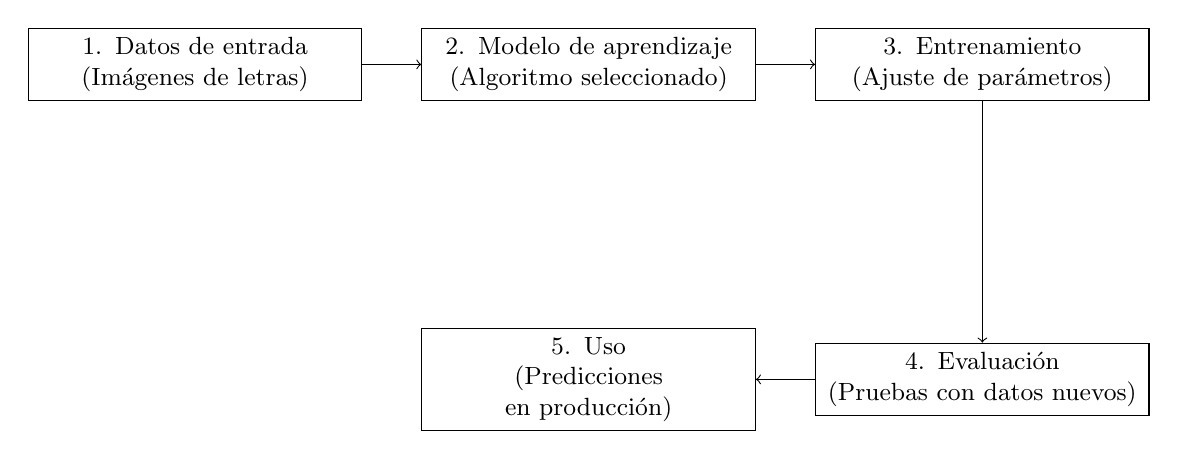
\begin{tikzpicture}[node distance=2cm, auto]
        % Nodes
    \node (data) [rectangle, draw, text width=4cm, align=center, font=\small] {1. Datos de entrada \\ (Imágenes de letras)};
    \node (model) [rectangle, draw, right of=data, xshift=3cm, text width=4cm, align=center, font=\small] {2. Modelo de aprendizaje \\ (Algoritmo seleccionado)};
    \node (training) [rectangle, draw, right of=model, xshift=3cm, text width=4cm, align=center, font=\small] {3. Entrenamiento \\ (Ajuste de parámetros)};
    \node (evaluation) [rectangle, draw, below of=training, yshift=-2cm, text width=4cm, align=center, font=\small] {4. Evaluación \\ (Pruebas con datos nuevos)};
    \node (deployment) [rectangle, draw, left of=evaluation, xshift=-3cm, text width=4cm, align=center, font=\small] {5. Uso \\ (Predicciones en producción)};


    % Arrows
    \draw[->] (data) -- (model) node[midway, above, font=\small] {};
    \draw[->] (model) -- (training) node[midway, above, font=\small] {};
    \draw[->] (training) -- (evaluation) node[midway, right, font=\small] {};
    \draw[->] (evaluation) -- (deployment) node[midway, below, font=\small] {};
    %\draw[->] (deployment.west) -- ++(-1.5,0) |- (data.west) node[midway, left] {Iteración};
\end{tikzpicture}

\end{document}

